\section{Software Implementation}
\fred is part of the \sksurgery\cite{PMID:32436132} family of libraries. In common with \sksurgery the majority of \fred is implemented in Python. Python was chosen as it combines sufficient features for clinical
applications, whilst remaining easy enough for students to learn and contribute to. A key design goal of 
\sksurgery is to keep individual libraries compact and atomic, simplifying dependency structures. Based on 
analysis using cloc\footnote{https://github.com/AlDanial/cloc [v1.82]} \fred consists of 802 lines of Python 
code. The user interface is implemented in HTML5 and JavaScript, enabling multiple simple deployment 
options. Again, using cloc, there are 561 lines of HTML5 and JavaScript.

Figure \ref{fig:dependencies} shows the direct dependencies of \fred. The key functional dependency is
\core\cite{matt_clarkson_2020_3965731}. \core implements matched point based registration \cite{Arun1987} together 
with the calculation of expected \gls{FLE} and \gls{TRE} (equations 10 and 31 from Fitzpatrick et al.\cite{Fitzpatrick1998}). Flask\footnote{https://palletsprojects.com/p/flask/ [v1.1.2]} provides the web application framework 
to enable the browser based user interface to communicate with the Python based back end. The user
interface communicates with the back end with a series of {POST} requests. All state information is stored in the 
browser front end, allowing the back end to remain stateless, simplifying deployment. 
Including the Google Cloud FireStore API\footnote{https://pypi.org/project/google-cloud-firestore/ [v2.0.1]} 
enables the optional storage of results in a remotely hosted database. Plotting functionality is implemented
using Chart.js\footnote{https://www.chartjs.org/ [v2.9.4]}

\begin{figure}
	\begin{center}
	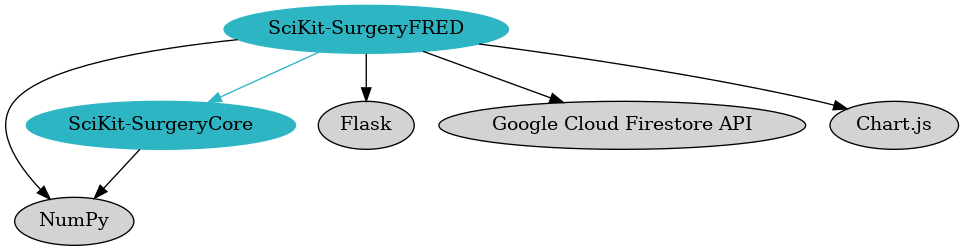
\includegraphics[width=0.7\linewidth]{dependency_graph.eps}
		\caption{\label{fig:dependencies}Software dependencies of SciKit-SurgeryFRED. The registration algorithms and statistical measures of {TRE} are imported from SciKit-SurgeryCore and are shared with clinical applications built on SciKit-Surgery. The user interface is implemented in HTML and JavaScript, using Chart.js for plotting functionality.}
	\end{center}
\end{figure}

